%!TEX root = ../../report.tex
\section{Accuracy and Precision of Localization with Dynamic Map}s
The effects of using a dynamic map representation for localization is evaluated by navigating precisely to the same pose multiple times using both a static and dynamic map representation.
By comparing how closely the robot gets to the target pose it is possible to evaluate the improvements in localization when using a dynamic map representation. 
\subsection{Test setup} 
The robot navigated along a path similar to the one shown in \ref{fig:amcl_covariance_static1} during a period of $35$ minutes using the static map representation and then the dynamic.
The robot stops in the lower left corner on the path during each cycle, where a camera is mounted parallel to and approximately $3.3$ meters above the floor.
The dynamic map is learned with the PMAC method described in this thesis while navigating with the static map for $35$ minutes.
\todo{consider inserting the path and where it stops}

The target pose is shown as a coordinate system in figure \ref{fig:mir_precision_explained}, where the robot is precisely located using a newly created map.
The pose of the chessboard relative to a camera posed above it is detected using MATLAB with the extrinsics function \cite{matlab_extrinsics} after calibrating the camera with MATLAB's Camera Calibrator App  \cite{camera_calibrator_app}.
The robot navigates with the planner in the MIR software, which stops when the estimated position is within one centimeter and the orientation is less than one degree of from target angle.

\begin{figure}
    \centering
    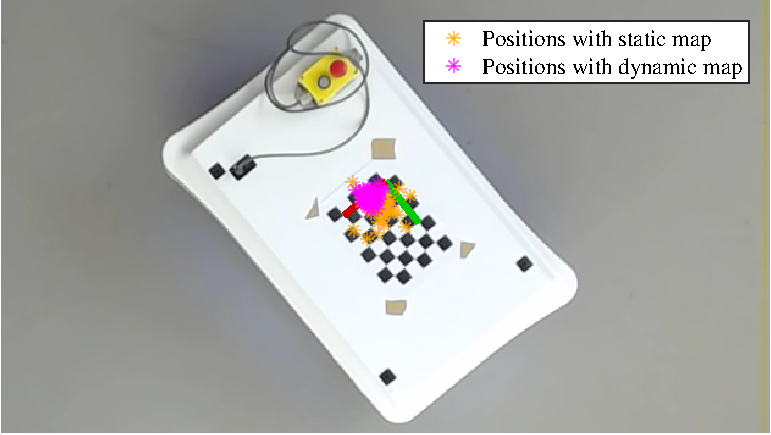
\includegraphics[scale=1]{chapters/evaluation/figures/mir_precision_explained}
    \caption{Image of MiR-100 at the target pose superimposed with the location of the marker frame and positions navigated to when attempting to get to the target.}
    \label{fig:mir_precision_explained}
\end{figure}

\subsection{Results}
The poses the robot navigates to while localizing on a static or dynamic map are compared on the amount they differ from the target pose.
Figure \ref{fig:precision_test_positions} shows the deviation in position using the dynamic map is less spread and that there is much less error in the y-direction. The mean error when using the static map is close to zero although the positions are widely spread.
This is confirmed with a one-sided F-test which shows that the variance in the x- and in the y-position is smaller when using a dynamic map representation than when using a static map with $p<0.001$ for both of them.
The improvements in accuracy when using a dynamic map is evident from the one-side Wilcoxon-test for equal median of the norm2 distance from the target position. The test shows that distance is significantly shorter with a $p<0.001$.

\begin{figure}
    \centering
    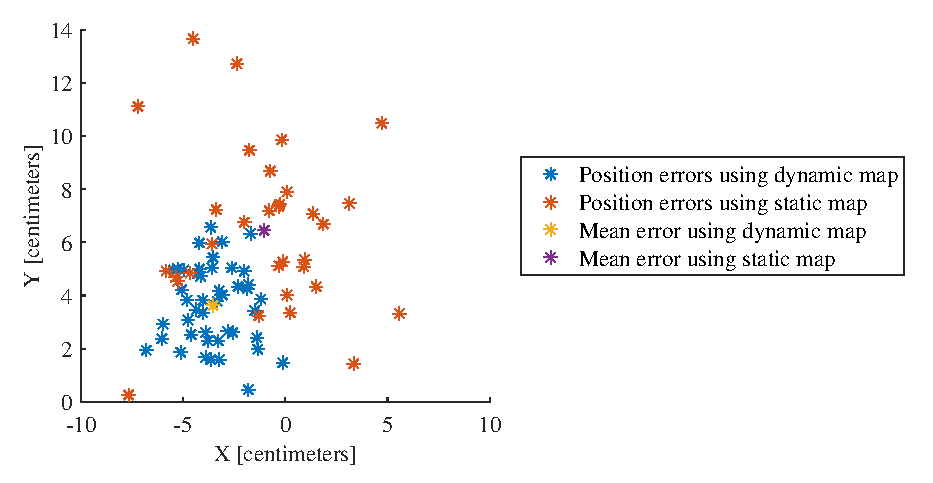
\includegraphics[scale=1]{chapters/evaluation/figures/precision_test_positions}
    \caption{Deviation in position from the target position.}
    \label{fig:precision_test_positions}
\end{figure}

There is less difference in the deviation in the angle from the target angle, as show in figure \ref{fig:precision_test_angles}. This is evident from the fact that the two-sided T-test showed that the Null-hypothesis of equal variance could not be rejected with $p=0.39$.
Considering that two-sided F-test shows that the variance in the orientation is not significantly different, it is clear that the precision is not improved significantly either.

\begin{figure}
    \centering
    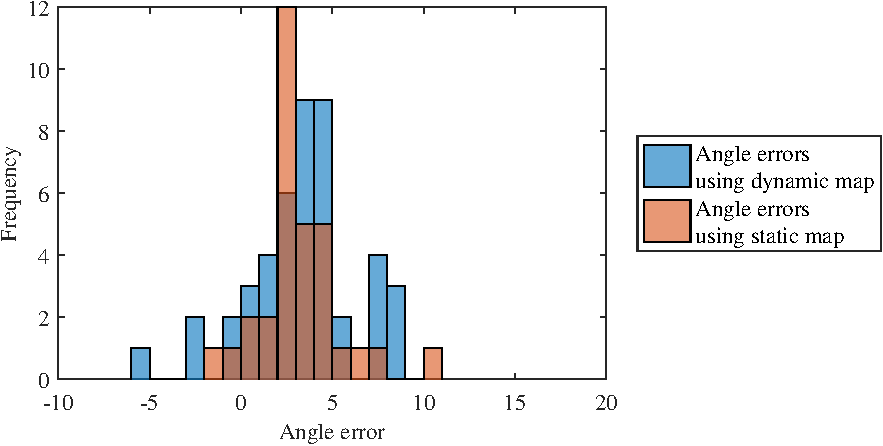
\includegraphics[scale=1]{chapters/evaluation/figures/precision_test_angles}
    \caption{Deviation in angle from the target angle.}
    \label{fig:precision_test_angles}
\end{figure}